\chapter{分光器の設計・製作}
前章で述べた通り,レンズを用いた同軸での集光は凹面鏡での軸外反射による集光と比べ高い集光性能を持つ.
そのため,凹面鏡によって集光する分光器と比べてレンズによって集光する分光器の方がより高い分解能を期待できる.
ただしレンズは色収差を持つため,レンズを用いた分光器では測定波長ごとにレンズの位置を変化させ検出器受光面に焦点を合わせる必要がある.

本研究ではコリメータ及び結像器にアクロマティックレンズ,検出器にはCCDカメラを用いる.
ここでより波長分散を大きくするために焦点距離が1525 mmと長焦点のアクロマティックレンズを使用する.
装置全体の大きさを小さく収めるために光路内に複数の平面ミラーを設置し光軸を折り曲げた設計とした.
設計波長域は400 nm~700 nmとした.

\section{分光器の設計}
\label{sec:spectrometer_design}
% 本研究ではコリメータ及び集光器にアクロマティックレンズ,検出器にはCCDカメラを用いる.
図\ \ref{fig:spectrometer_design}に設計した分光器の概略図を示す.
\begin{figure}[htbp]
    \centering
    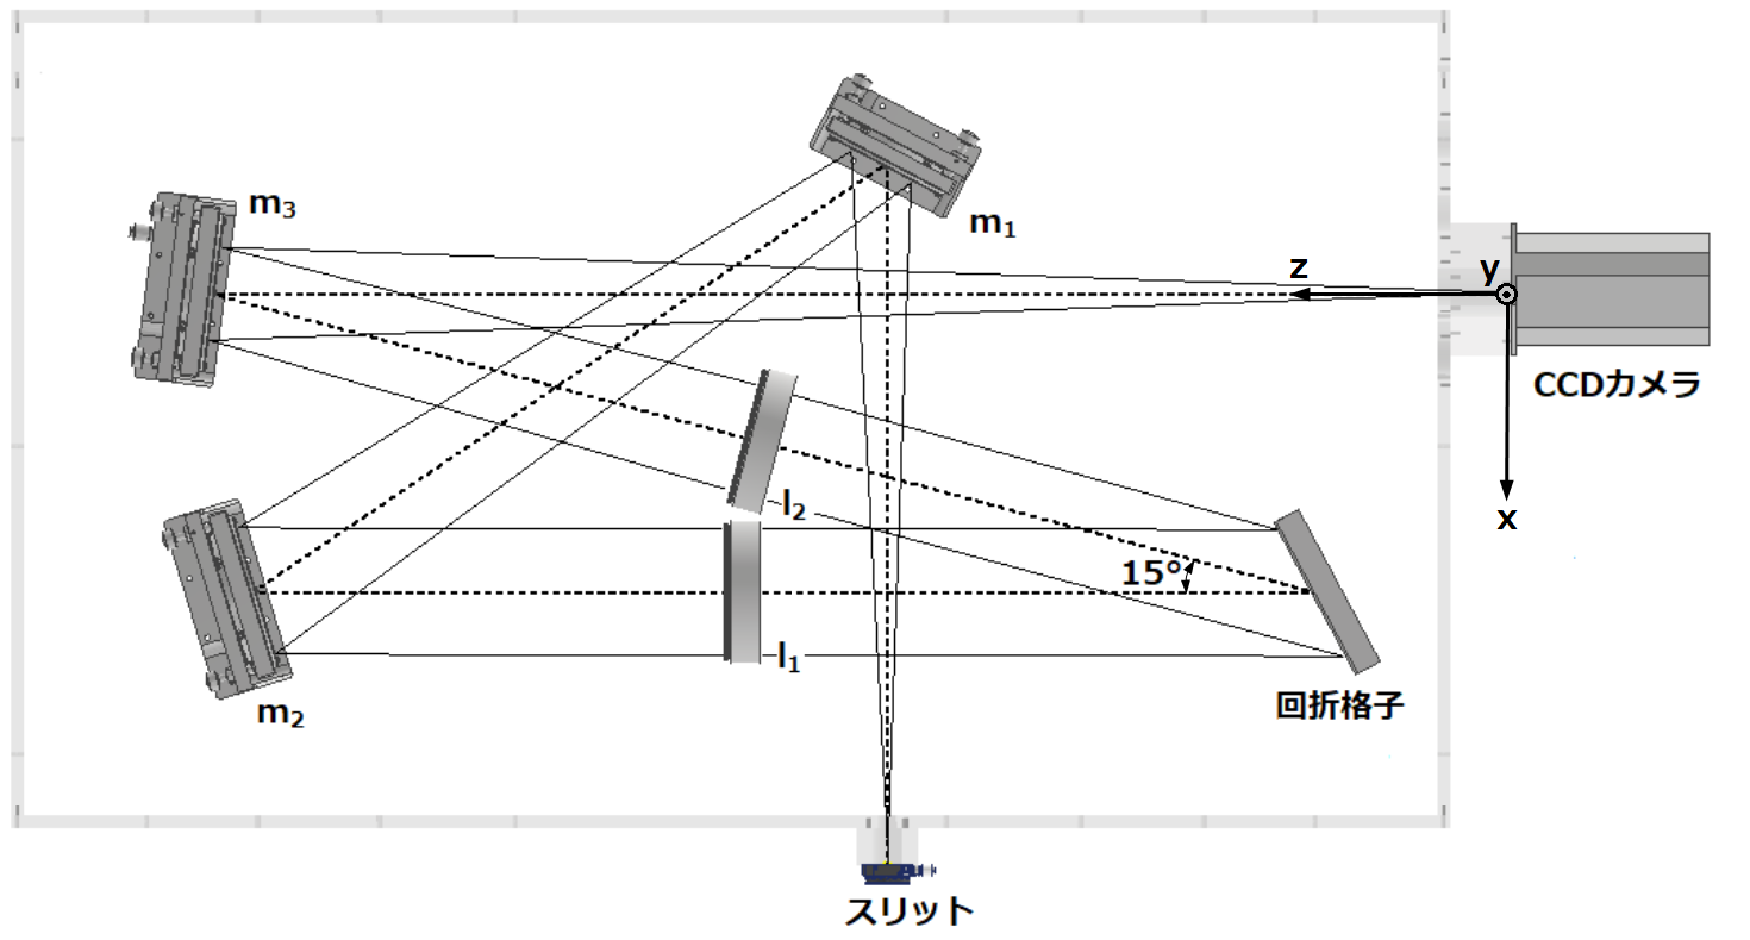
\includegraphics[scale=0.55]{figure/spectrometer_design2.pdf}
    \caption{分光器概略図}
    \label{fig:spectrometer_design}
\end{figure}
入口スリット(スリット幅10 $\mu$m)から入射された光は平面鏡$\mathrm{m_1}$(有効径77 mm)及び平面鏡$\mathrm{m_2}$(有効径96 mm)に反射した後,レンズ$\mathrm{l_1}$(Edmund Optics TS 大口径アクロマティックレンズ $\#$54568,焦点距離1525 mm,有効径98 mm)によって平行光に変えられる.
平行光は回折格子(2400 grooves/mm,$112\times132$ $\mathrm{mm^{2}}$)によって回折される.
その後,レンズ$\mathrm{l_2}$(焦点距離1525 mm,有効径98 mm)を通ることで集光され,平面鏡$\mathrm{m_3}$(有効径96 mm)によって反射された後,検出器であるCCDカメラ(ANDOR DV435,13×13 $\mu\mathrm{m^{2}}$/ピクセル,1024×1024 ピクセル,16 bit)に結像される.
% ここでレンズは球面収差をより抑えるために焦点距離が1525 mmと長いアクロマティックレンズを使用している.
% 装置全体の大きさを小さく収めるために光路内に複数の平面ミラーを設置し光軸を折り曲げた設計とした.
なお,便宜上CCDカメラの受光部の中心を原点に図のように座標系を設定する.

図\ \ref{fig:lens_grating_system}(a)(b)にレンズ及び回折格子周りの各部品の配置を示す.
\floatsetup[figure]{style=plain,subcapbesideposition=top}
\begin{figure}
    \sidesubfloat[]{
        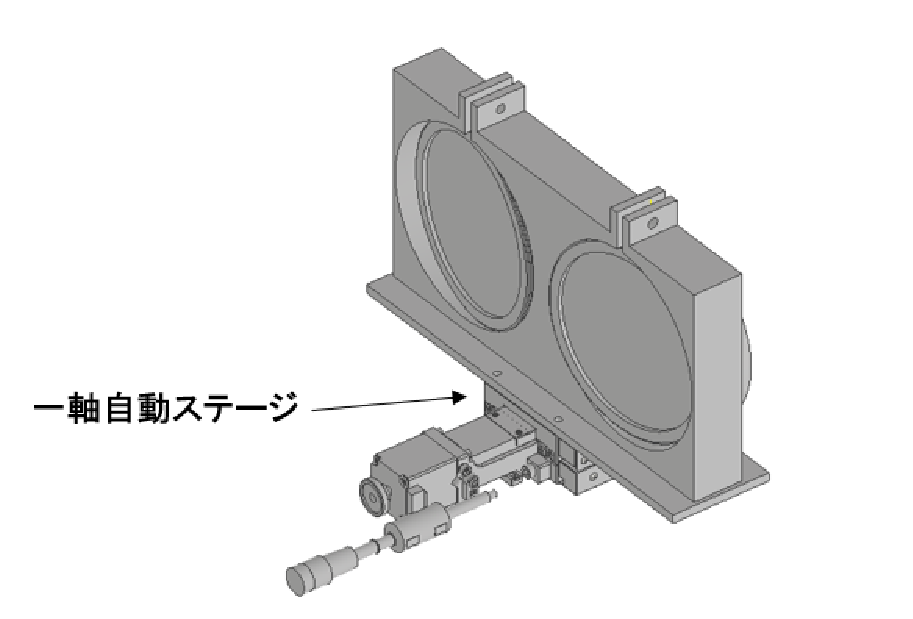
\includegraphics[scale=0.5]{figure/lense_system.pdf}}
    \sidesubfloat[]{
        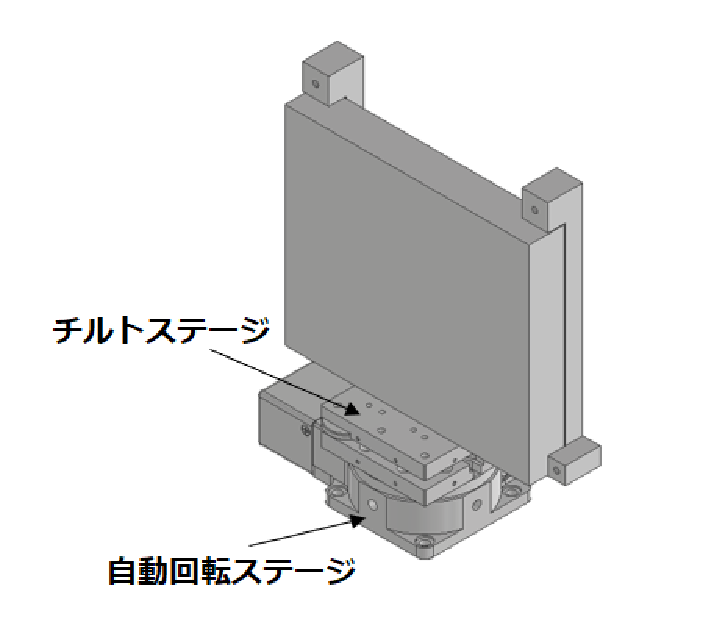
\includegraphics[scale=0.5]{figure/grating_system.pdf}}
    \caption{(a)レンズ周りの部品構成,(b)回折格子周りの部品構成}
    \label{fig:lens_grating_system}
\end{figure}
二つのレンズはレンズホルダによって固定している.
フォーカス調整のためにレンズの下に一軸自動ステージ(シグマ光機株式会社製 HPS60-20X-M5,1 $\mu\mathrm{m}$/パルス,移動量$\pm{10.0}$ mm)を取り付けた.
また,回折格子の下には水平方向の傾きを微調整するためのチルトステージと回折格子の角度(回折格子の面の向き)を制御するための自動回転ステージ(シグマ光機株式会社製 OSMS-60YAW,0.0025°/パルス)を取り付けた.
これらの自動ステージはそれぞれのステージのステッピングモータに入力されるパルス信号で制御されている.
以下では回転ステージ,一軸自動ステージのパルスの絶対値をそれぞれ回折格子パルス,フォーカスパルスと呼ぶこととする.
さらに,レンズ下の一軸自動ステージの移動量が足りない場合を想定して,平面鏡$\mathrm{m_3}$の下には一軸手動ステージ(シグマ光機株式会社製 TSD-601S,移動量$\pm{6.5}$ mm)を取り付けた.
またスリットと分光器筐体の間に取り付けたスリット台の厚みを変えることでスリットのx軸方向の位置を任意に変更できるようにした.

% \floatsetup[figure]{style=plain,subcapbesideposition=top}
% \begin{figure}
%     \sidesubfloat[]{
%         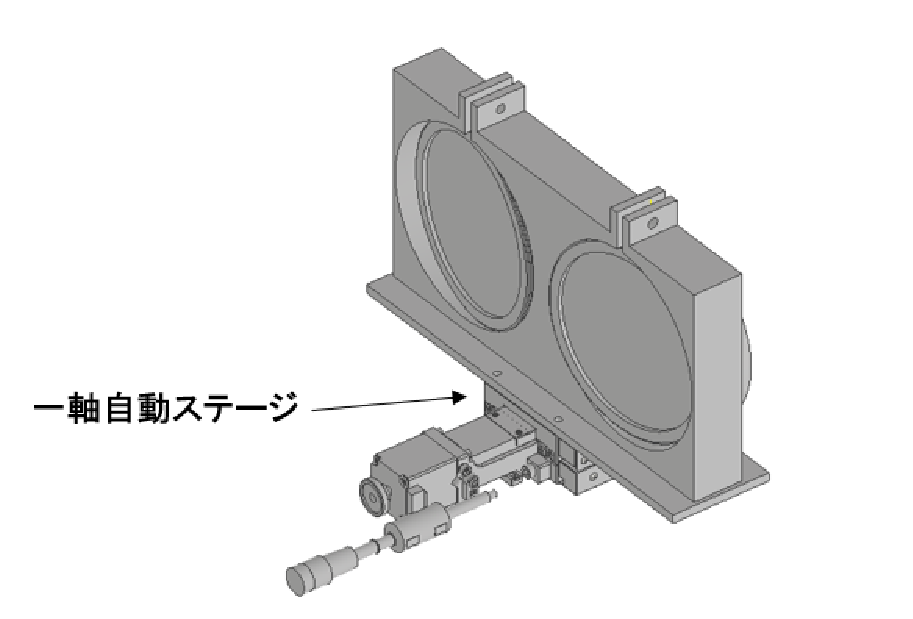
\includegraphics[scale=0.5]{figure/lense_system.pdf}}
%     \sidesubfloat[]{
%         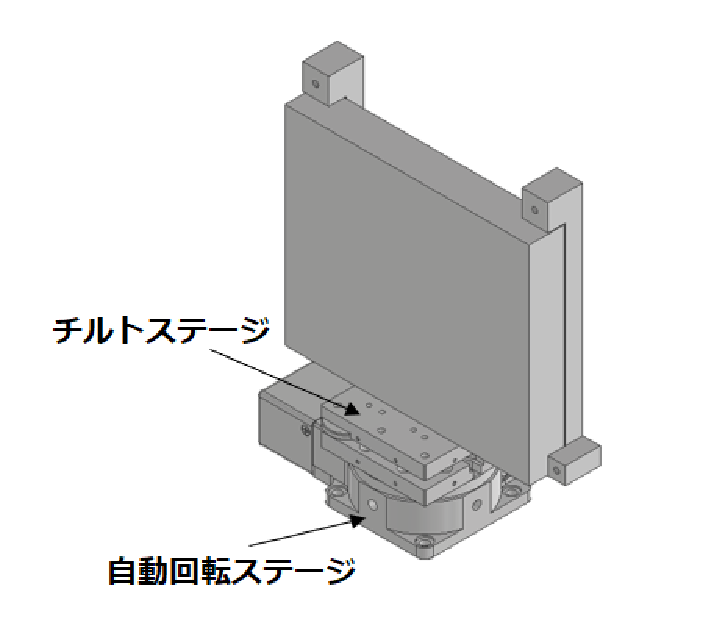
\includegraphics[scale=0.5]{figure/grating_system.pdf}}
%     \captionsetup{
%     (a):レンズ周りの部品構成
%     (b):回折格子周りの部品構成}
%     \label{fig:lense_grating_system}
% \end{figure}

% 本研究では分光器の入口スリットは幅10 $\mu$mのものを使用しているため,CCDカメラの結像面でも10$\mu$mの幅で結像されること期待して設計している.
% それを実現するためには,レンズが直径10$\mu$m以下の大きさに光を結像できる性能を持っている必要がある.
% 使用レンズを用いた際のスポットの様子を確認するためにOSLOを用いてシミュレーションを行った.
% Fig.\ \ref{fig:lens_spot}は今回使用するレンズに波長587.6nmの平行光を入射したときのスポット図を表す.
% \begin{figure}[htbp]
%     \centering
%     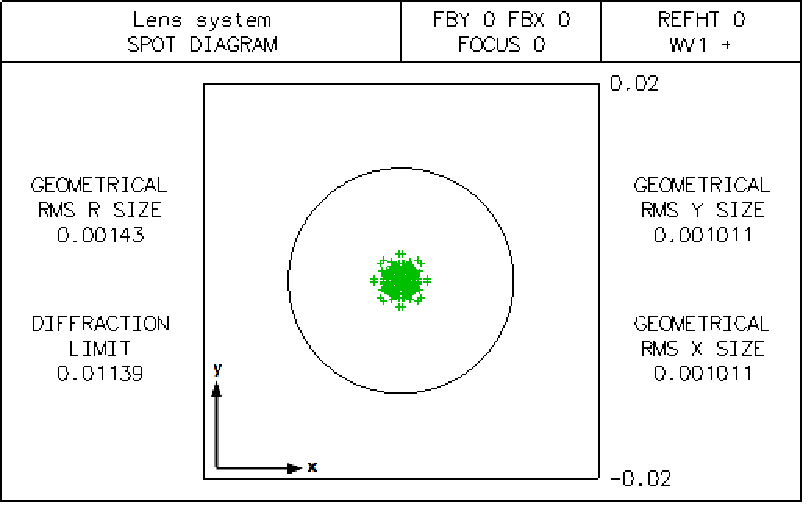
\includegraphics[scale=0.6]{figure/lens_spot.pdf}
%     \caption{波長587.6nmの光を垂直に入射させたときの使用レンズのスポット図}
%     \label{fig:lens_spot}
% \end{figure}
% 全ての光線がエアリーディスク内に収まっており結像の大きさが回折限界によって制限されていることが分かる.

今回二つのレンズを一つのステージでまとめて移動させるように設計したため,各レンズは光軸方向とわずかにずれて移動する.
そのため一軸自動ステージの移動量が大きいほどレンズは光軸から傾く.
一軸自動ステージの移動量の範囲では,最大で約0.16°傾く.

このレンズの傾きによる影響を検証するためにOSLOを用いて結像の様子をシミュレーションした.
レンズに0.16°傾いた光を入射させたときの焦点面でのスポット図を図\ \ref{fig:lens_spot_zure}に示す.
\begin{figure}[htbp]
    \centering
    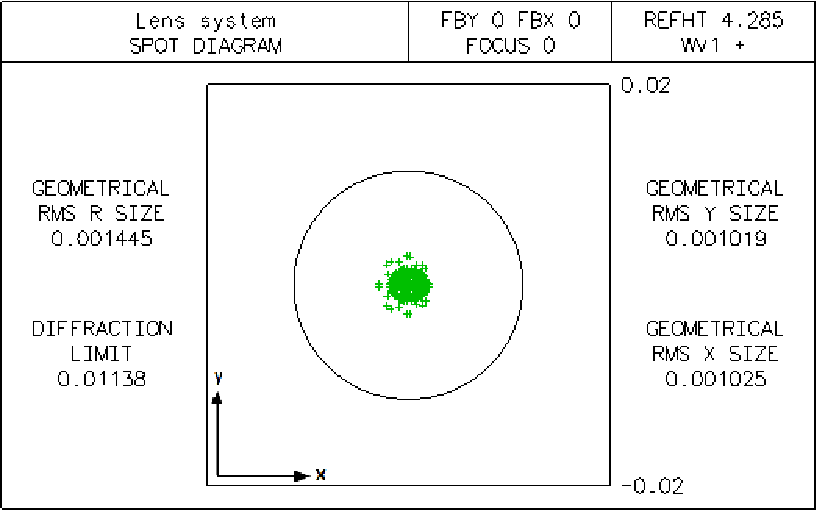
\includegraphics[scale=0.6]{figure/lens_spot_zure.pdf}
    \caption{本分光器の使用レンズに光を0.16°傾けて入射させたとき焦点面でのスポット図}
    \label{fig:lens_spot_zure}
\end{figure}
図から分かるようにすべての光線がエアリーディスク内に収まっていることから0.16°光が傾いて入射しても回折限界で集光できる.
従って,このレンズの傾きによって生まれる収差の影響は小さいと言える.

\section{装置幅の予測}
分光器に単波長の光を入射させたとしても,スペクトルは収差やスリット幅に依存した有限の幅を持つ.
この各分光器ごとに固有であるスペクトルの幅を装置幅と呼ぶ.
設計した分光器の理論的な装置幅を求めるため,設計波長域において装置幅に影響を与えるスリット幅,レンズの収差,回折限界からくる波長幅を比較する.

回折限界における理論的なスペクトルの最小波長幅
\begin{equation}
     \delta\lambda = \frac{0.99 \lambda \mathrm{cos}{\beta} }{mNW}
\end{equation}
及びスリット幅$s$=10 $\mu$mから入った光が理想的に結像された際のスペクトルの波長幅
\begin{eqnarray}
     d\lambda &=& 
        \frac{s\mathrm{cos}^2{\beta}}{Nmf\mathrm{cos}{\alpha}}
\end{eqnarray}
及び使用レンズがつくる設計上の結像の大きさに対応する波長幅を表すものを図\ \ref{fig:instrumental_function_design}に示す.
\begin{figure}[htbp]
    \centering
    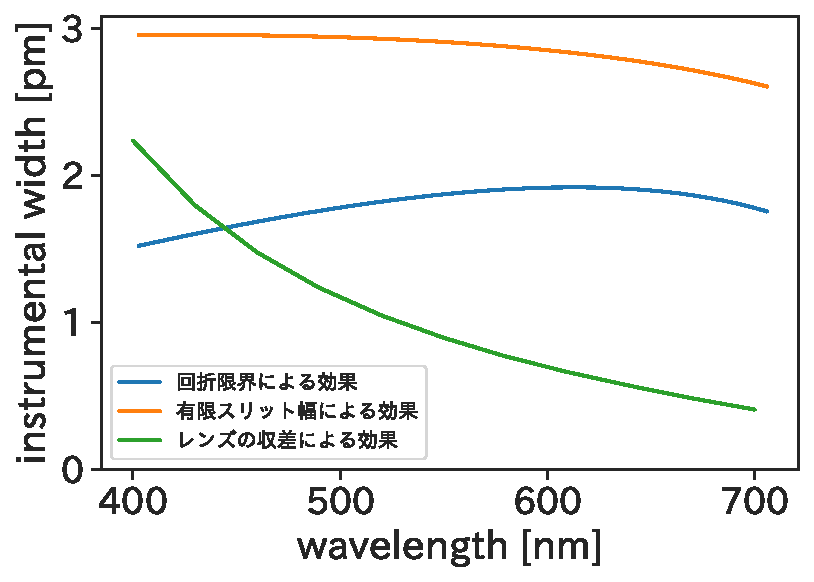
\includegraphics[scale=0.7]{figure/instrumental_function_design.pdf}
    \caption{装置幅に影響を与える要素による波長幅の比較}
    \label{fig:instrumental_function_design}
\end{figure}
% 線1が回折格子の理論分解能,線2が本分光器においてスリット幅の効果で結像されたときの波長幅,線3が使用レンズのスポットサイズに対応する波長幅を表す.
% ここで理想的に結像された際の波長幅とはスリットの幅10 $\mu$mから入射された光が回折格子によって$d\alpha/d\beta$倍に拡大され結像するとした際のスペクトルの波長幅のことでスリット幅s×拡大率の大きさ($|d\alpha/d\beta|$)×逆線分散($d\lambda/dx$)となり以下の式で表される.
% \begin{eqnarray}
%      d\lambda &=& s\left|\frac{d\alpha}{d\beta}\right|\frac{d\lambda}{dx} \\
%         &=&s\frac{\mathrm{cos}{\beta}}{\mathrm{cos}{\alpha}}\frac{\mathrm{cos}{\beta}}{Nmf} \\
%         &=&\frac{s\mathrm{cos}^2{\beta}}{Nmf\mathrm{cos}{\alpha}}
% \end{eqnarray}
使用レンズのつくる設計上の結像の大きさはOSLOを用いて使用レンズに波長400 nmから30 nm間隔で波長700 nmまでの光を入射させた際の焦点面でのスポット図をシミュレーションし,それぞれの$\phi$とした.


図\ref{fig:instrumental_function_design}において回折限界での波長幅及び使用レンズの作る設計上の結像の大きさに対応する波長幅は設計波長域で常にスリット幅10 $\mu$mから入った光が理想的に結像された際の波長幅より小さい.
よって今回の設計において,分光器の装置幅は主にスリット幅によるものであり,レンズの球面収差や回折限界による影響は受けにくいと期待される.


% そこから,本研究では設計波長域においてFig.\ \ref{fig:instrumental_function_design}中の線2に迫る$3.0\times10^{-3}$ nmの装置幅を目指して分光器を製作した.



\section{光学配置の調整}
% 筐体に各部品を取り付けるだけではCCDカメラの受光部に正確に焦点は合わず,各部品の位置・角度の微調整を要する.
% 調整は大きく分けて焦点位置の鉛直方向の調整とフォーカスの調整とがある.



\subsection{結像位置の調整}
xy平面上において結像位置がCCDカメラの受光部からy軸方向にずれていると,いくら回折格子を回転させてもCCDカメラに発光線は映らない.
そこで光源にHeNeレーザー(波長632.8 nm)を用いて,CCDカメラの中心部に結像位置が来るように各ミラー及び回折格子の傾きを調整した.

分光器の設計ではy=0の面に対して対称になるような光学系の配置であるため,回折格子の角度に関係なく結像位置のy座標は全ての発光線において変化しないはずである.
しかし回折格子が水平でなく,入射光と回折格子の刻線に垂直な面に傾きがある場合,対称性が失われ回折格子の角度によって結像位置のy座標は変化してしまう.
そこで今回,回折格子の傾きを直すためHeNeレーザーの$\pm{}$1次光及び0次光の結像位置のy座標の位置を揃えるように調整した.


% これは回折格子の角度によって発光線のy軸方向の結像位置が変化しているということである.
% しかし,今回の分光器の設計ではy=0の面に対して対称になるような光学系の配置であるため,設計通りであればこのような現象は起こりえない.
% 従ってこの現象は回折格子が水平でなく,入射光と回折格子の刻線に垂直な面に傾きあるために生じるものであると考え,それぞれの発光線のy軸方向の位置が揃うようにした.

% そのため,それぞれのスペクトルの高さが揃うようにした.

%  また,平面鏡$m_3$の下の一軸手動ステージを調節しCCDカメラの受光面に焦点が来るように調節を試みた.しかし,一軸手動ステージの移動量では限界があったため,スリットと分光器の筐体の間に3Dプリンタで作成した台を入れることによりさらなる調整を可能にしたd.
\subsection{結像のフォーカス調整}
分光器の分解能を高めるためには発光線をできるだけ細く結像させる必要がある.
従って,レンズの焦点距離にCCDカメラの受光面を正確に合わせるべきである.
結像位置の調整と同じく光源にHeNeレーザーを用いて発光線がCCDカメラ中心になるように回折格子パルスを設定し,フォーカスパルスを等間隔で変化させて31個のデータを撮影した.
図\ \ref{fig:HeNe_focus_example}は撮影した各データにおけるフォーカスパルスとスペクトル幅の関係性を表している.
\floatsetup[figure]{style=plain,subcapbesideposition=top}
\begin{figure}
    \sidesubfloat[]{
        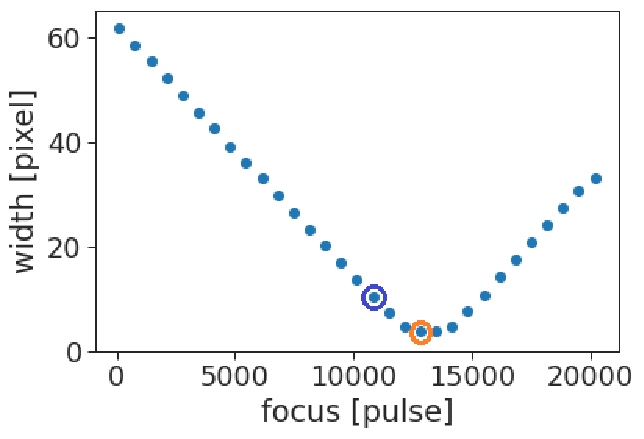
\includegraphics[scale=0.6]{figure/HeNe_focus_example.pdf}}
    \sidesubfloat[]{
        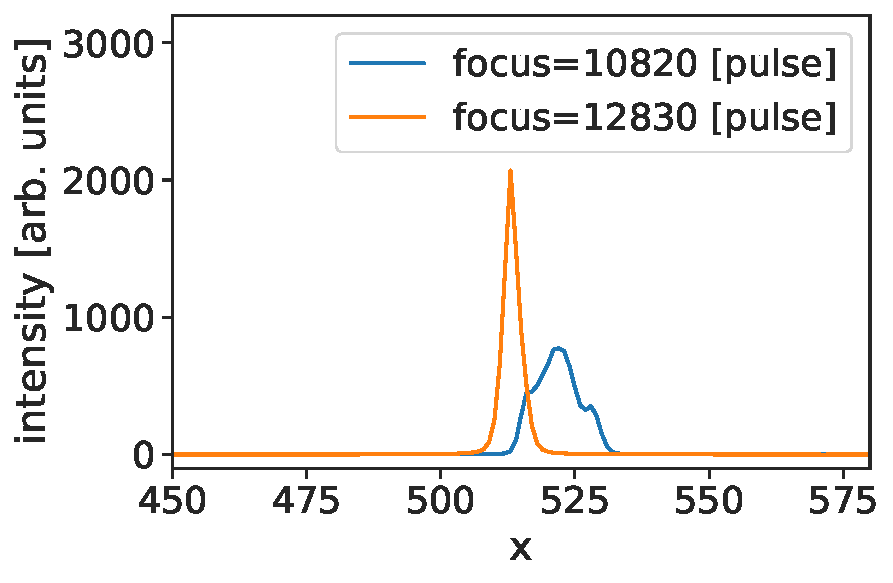
\includegraphics[scale=0.45]{figure/HeNe_focus_example_comparison.pdf}}
    \caption{
    (a)HeNeレーザ光源でのフォーカスパルスの変化とスペクトル幅の関係.オレンジで囲った点は最も焦点が合っているフォーカスパルスが12830のものを示している,
    (b)フォーカスパルスが10820のときと12830のときに得られたスペクトル}
    \label{fig:HeNe_focus_example}
\end{figure}
ここでスペクトル幅は撮影したデータをy軸方向に足し合わせて作成したスペクトル図をガウス関数でフィッティングした際の半値全幅とした.
スペクトル幅が最小値を取る時が焦点が合っている時であるといえる.

% 実際の分光計測で用いるのは焦点があっている時のスペクトルのみである.
% 合焦時のスペクトル幅をより小さくできないかと考え,平面鏡$\mathrm{m_3}$の下に取り付けた一軸手動ステージ及びスリット台の厚さを変更しながらそれぞれで最小スペクトル幅を求めた.
% しかし平面鏡$\mathrm{m_3}$の位置,スリット台の厚さを変えても焦点が合っている時のスペクトル幅は大きくは変わらず,それらの相関関係を見つけることはできなかった.


% % $\pm{1}$次光のスペクトルを観測したとき焦点が合っているフォーカスパルスの値がずれがあった.
% Figure\ \ref{fig:HeNe_focus}(a)にその一例を示す.
% 波長が同じなら色収差による焦点距離の変化は発生しないため,1次光でも-1次光でも関係なくフォーカスの位置は一致するはずである.


% この現象は回折格子に入射する光が平行光でなかった,つまりレンズ$\mathrm{l_1}$とスリット間の距離が焦点距離からずれていたためである.
% 入射光が平行でないということは幅のある入射角で回折格子に入射していると言い換えられる.
% ここで,入射角が$\alpha$から$\alpha+\delta\alpha$までの幅を持っており,入射角$\alpha$,$\alpha+\delta\alpha$に対応する回折角を$\beta$,$\beta+\delta\beta$となるとすると
% \begin{eqnarray}
%     Nm\lambda &=& \mathrm{sin}{\alpha}+\mathrm{sin}{\beta} \\
%     Nm\lambda &=& \mathrm{sin}{(\alpha+\delta\alpha)}+\mathrm{sin}{(\beta+\delta\beta)}
% \end{eqnarray}
% とでき,$\delta\alpha$,$\delta\beta$が微小であるとして$\mathrm{sin}{\delta\alpha}=\delta\alpha,\mathrm{sin}{\delta\beta}=\delta\beta$,$\mathrm{cos}{\delta\alpha}=\mathrm{cos}{\delta\beta}=1$と近似して計算すると,
% \begin{eqnarray}
%     \delta\alpha=-\frac{\mathrm{cos}{\beta}}{\mathrm{cos}{\alpha}}\delta\beta
% \end{eqnarray}
% ここで,$(-\mathrm{cos}{\beta}/\mathrm{cos}{\alpha})$は回折格子の拡大率であり,$\pm{}$1次光で拡大,縮小が反転される.
% したがって,$\delta\alpha$に対応する$\delta\beta$の値は$\pm{}$1次光で異なる.
% これらより回折格子に非平行光が入射したとき,$\pm{}$1次光で回折光の広がり方が異なり,焦点距離が変化する.


% 本研究では回折格子には平行光を当てることを前提に設計していたので,$\pm{1}$次光のスペクトルで焦点の合うフォーカスパルスが一致するように各光学素子を調整した.
% % この際,平面鏡$m_3$の下の一軸手動ステージだけでは光軸方向の変化量が不足していたため,スリットと分光器の筐体の間に3Dプリンタで作成した台を入れることによりさらなる調整を可能にした.
% % スリットの台は厚さ5mmのものから5mmずつ厚くしてゆき最大で厚さ30mmのものまで作成した.
% Figure.\ \ref{fig:HeNe_focus}(b)で平面鏡$m_3$を元の位置から6.5 mm前にし,30 mmの厚さのスリット台を使用して撮影した際の$\pm{1}$次光のスペクトル幅とフォーカスパルスの関係性を示す.
% 図より波長が632.8 nmの時$\pm{1}$次光で焦点が合うフォーカスパルスの値が9500ほどで揃っていることが分かる.
% \floatsetup[figure]{style=plain,subcapbesideposition=top}
% \begin{figure}
%     \sidesubfloat[]{
%         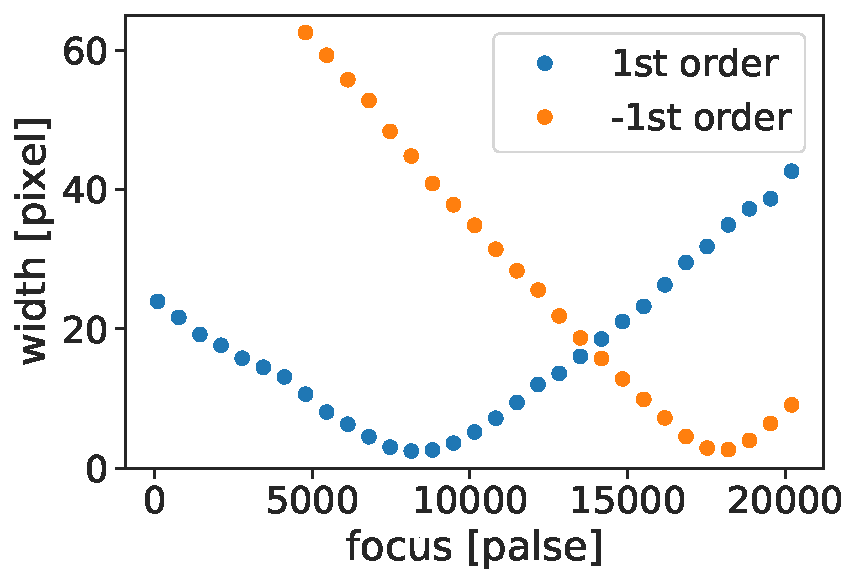
\includegraphics[scale=0.45]{figure/HeNe_focus_before.pdf}}
%     \sidesubfloat[]{
%         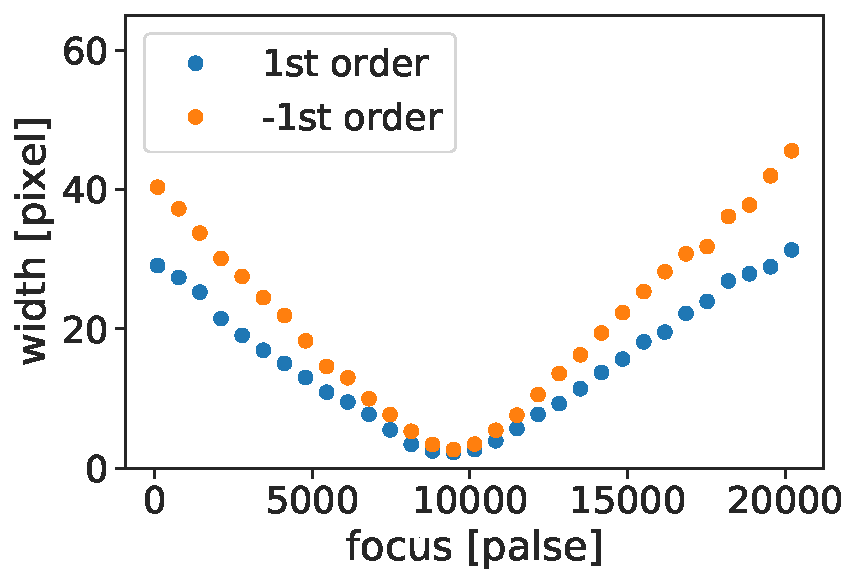
\includegraphics[scale=0.45]{figure/HeNe_focus_after.pdf}}
%     \caption{HeNeレーザを光源にした際の$\pm{1}$次光のスペクトル幅とフォーカスパルスの関係性
%     (a):平面鏡$\mathrm{m_3}$の位置はそのままでスリット台は10mmのものを使用して撮影
%     (b):平面鏡$\mathrm{m_3}$の位置を6.5mm前にしスリット台は30mmのものを使用して撮影}
%     \label{fig:HeNe_focus}
% \end{figure}


% ここから下
本分光器はレンズ$\mathrm{l_1}$とスリット間の距離をレンズの焦点距離にすることで,レンズ$\mathrm{l_1}$に入射する光を平行光にしている.
また同様にレンズ$\mathrm{l_2}$とCCDカメラの受光面の距離をレンズの焦点距離にすることで平行光をレンズ$\mathrm{l_2}$に入射したしたときCCDカメラの受光面に結像されるようにしている.
しかし,レンズ$\mathrm{l_1}$とレンズ$\mathrm{l_2}$をまとめて動かすよう設計しているので平面鏡$\mathrm{m_3}$及びスリットの位置を適切に設定しないと,レンズ$\mathrm{l_1}$とスリットの間の距離,レンズ$\mathrm{l_2}$とCCDカメラ受光面の距離の両方を同時に焦点距離に合わせることはできない.
よってCCDカメラ受光面に焦点が合うように調整されていても,レンズ$\mathrm{l_1}$とスリット間の距離が適切でなく平行光にできていない場合が存在する.
ここで,回折格子に非平行光が入射した際について考える.
入射角が$\alpha$から$\alpha+\delta\alpha$までの幅を持っており,入射角$\alpha$,$\alpha+\delta\alpha$に対応する回折角をそれぞれ$\beta$,$\beta+\delta\beta$となるとすると
\begin{eqnarray}
    Nm\lambda &=& \mathrm{sin}{\alpha}+\mathrm{sin}{\beta} \\
    Nm\lambda &=& \mathrm{sin}{(\alpha+\delta\alpha)}+\mathrm{sin}{(\beta+\delta\beta)}
\end{eqnarray}
とできる.
$\delta\alpha$,$\delta\beta$が微小であるとして$\mathrm{sin}{\delta\alpha}\simeq\delta\alpha,\mathrm{sin}{\delta\beta}\simeq\delta\beta$,$\mathrm{cos}{\delta\alpha}\simeq\mathrm{cos}{\delta\beta}\simeq1$と近似して計算すると,
\begin{eqnarray}
    \delta\alpha\simeq-\frac{\mathrm{cos}{\beta}}{\mathrm{cos}{\alpha}}\delta\beta
\end{eqnarray}
が求められる.
ここで,$-\frac{\mathrm{cos}{\beta}}{\mathrm{cos}{\alpha}}$は回折格子での拡大率であり,本分光器では+1次光で$|\frac{\mathrm{cos}{\beta}}{\mathrm{cos}{\alpha}}|>1$であり像は拡大,-1次光で$|\frac{\mathrm{cos}{\beta}}{\mathrm{cos}{\alpha}}|<1$であり像は縮小する.
$\delta\alpha$に対応する$\delta\beta$の値は$\pm{}$1次光で異なることから,回折格子に非平行光が入射した場合$\pm{}$1次光で回折光の広がり方が異なることになり,結果としてレンズで集光する際の焦点位置が変化する.
平面鏡$\mathrm{m_3}$及びスリットの位置が適切でないと同波長の$\pm{1}$次光のスペクトルを観測する際,CCDカメラ受光面に焦点が合うフォーカスパルスの値にずれが生じる.
図\ \ref{fig:HeNe_focus}(a)にその一例を示す.
これは平面鏡$\mathrm{m_3}$が初期位置で10 mmの厚さのスリット台を使用した際の$\pm{1}$次光におけるフォーカスパルスとスペクトル幅を表している.

回折格子に平行光が入射されるようにするため$\pm{1}$次光のスペクトルで焦点の合うフォーカスパルスが一致するように各光学素子を調整した.
図\ \ref{fig:HeNe_focus}(b)に平面鏡$\mathrm{m_3}$を初期位置から6.5 mm前にし,30 mmの厚さのスリット台を使用して撮影した際の$\pm{1}$次光のフォーカスパルスとスペクトル幅の関係性を示す.
図より波長が632.8 nmの時$\pm{1}$次光で焦点が合うフォーカスパルスの値が9500ほどで揃っていることが分かる.
これによってスリット,及び各平面鏡が正しい位置に配置され,回折格子に平行光が入射されていることが確認できた.
\floatsetup[figure]{style=plain,subcapbesideposition=top}
\begin{figure}
    \sidesubfloat[]{
        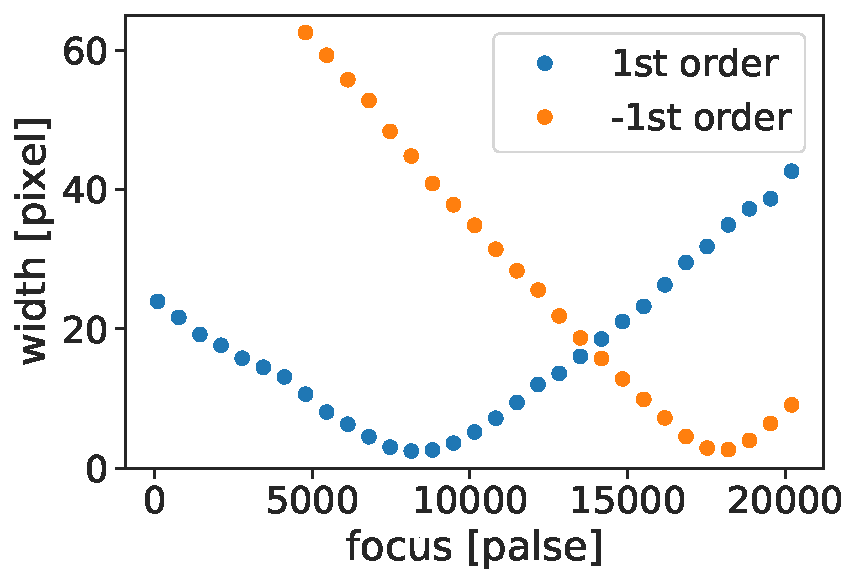
\includegraphics[scale=0.45]{figure/HeNe_focus_before.pdf}}
    \sidesubfloat[]{
        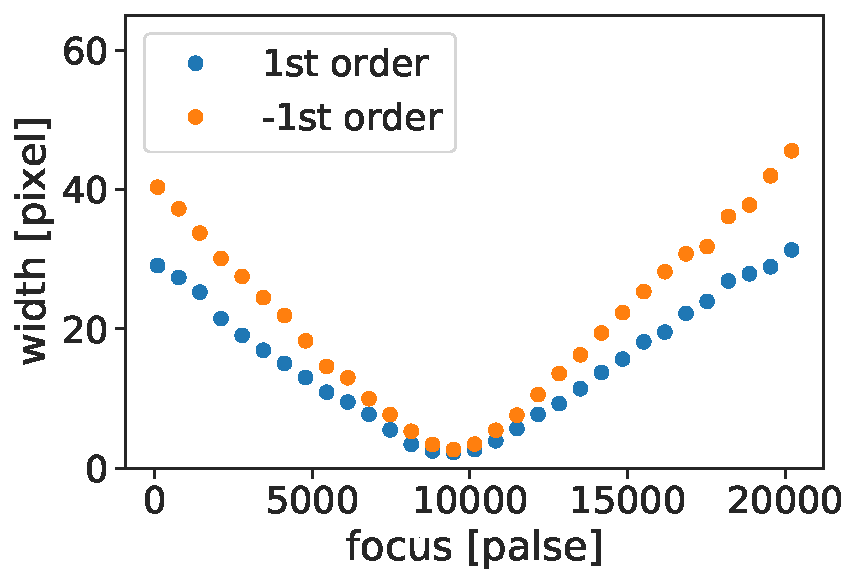
\includegraphics[scale=0.45]{figure/HeNe_focus_after.pdf}}
    \caption{HeNeレーザを光源にした際の$\pm{1}$次光のスペクトル幅とフォーカスパルスの関係性
    (a)平面鏡$\mathrm{m_3}$は初期位置のままで10 mmの厚さのスリット台を使用して撮影,
    (b)平面鏡$\mathrm{m_3}$の位置を初期位置から6.5 mm前にし30 mmの厚さのスリット台を使用して撮影}
    \label{fig:HeNe_focus}
\end{figure}

\subsection{迷光除去}
% 弱いスペクトルを計測しようとしたとき,画面左下側の光の強度が高くなる傾向があることが分かった.
% そのため,目的の波長以外の光が何らかの形でCCDカメラに入ってしまっていると考えた.
図\ \ref{fig:meikou}(a)はスリットに光を入れないで撮影した際のCCDカメラ受光部の光の強度分布である.
図よりCCDカメラの受光部において左下側にわずかに光が当たっていることが分かる.
この光はレンズ下の一軸自動ステージにリミットセンサとして取り付けられているフォトインタラプタによるものである.
このような本来の光路外から発生した光のことを迷光と呼ぶ.
迷光は正確な分光測定を阻害する要因となるため,除去することが望ましい.

CCDカメラに迷光が入らないようにするため,CCDカメラ入口近くに簡易的な遮光壁を光路を遮らないよう設置した(図\ \ref{fig:syakouban}).
\begin{figure}[htbp]
    \centering
    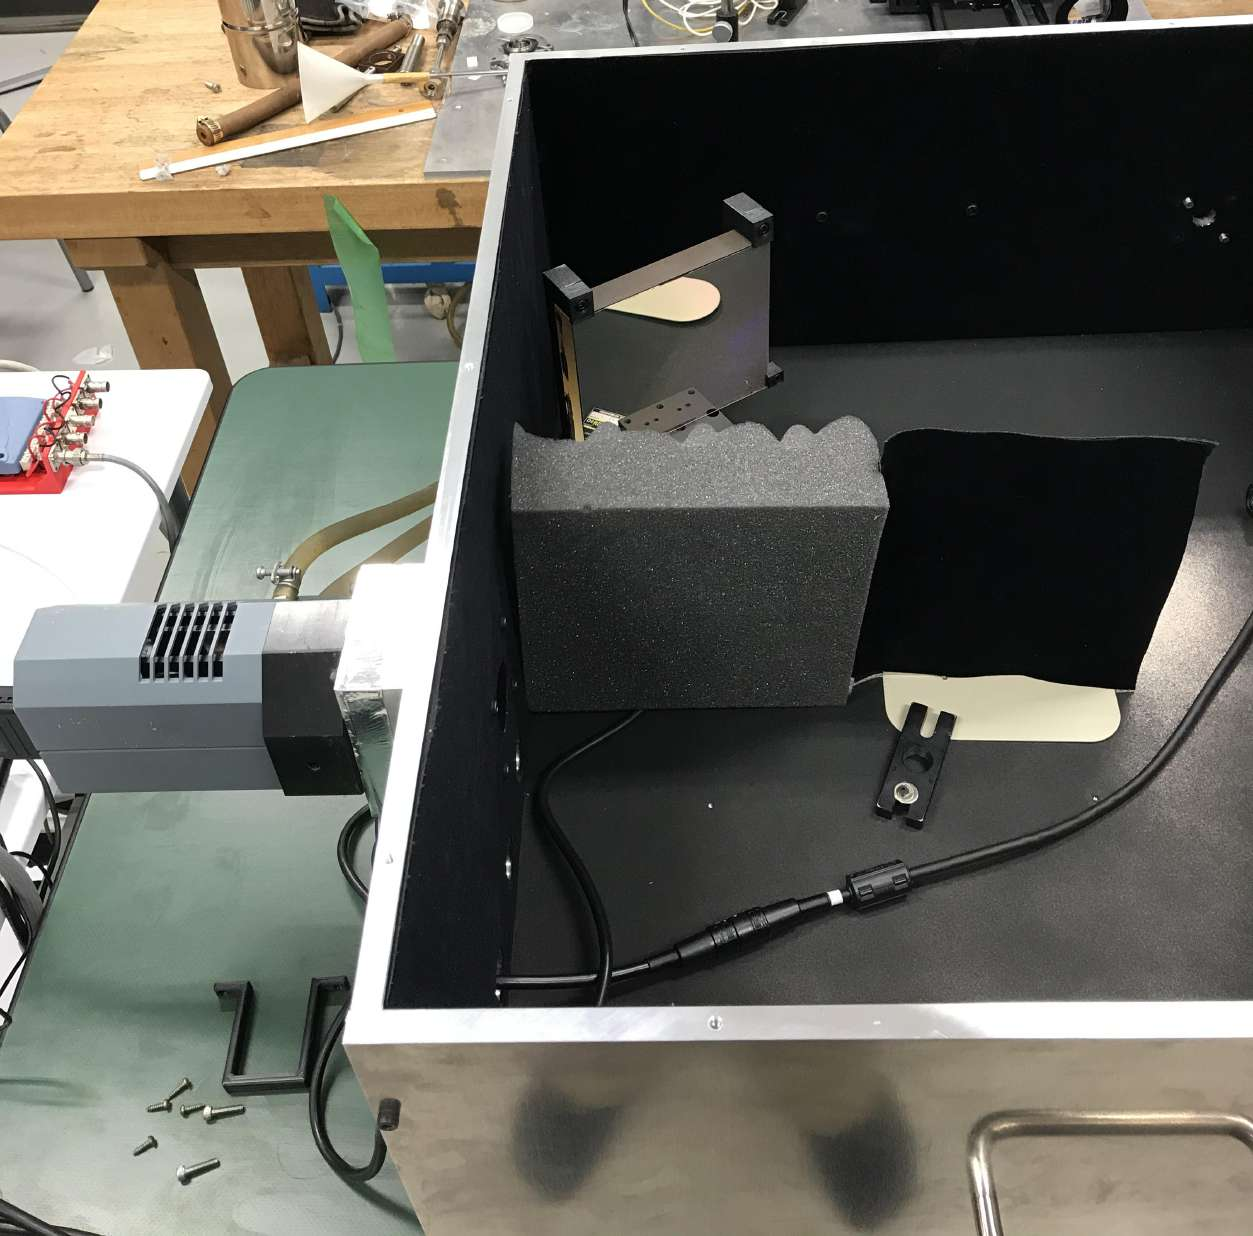
\includegraphics[scale=0.3]{figure/syakouban_compressed.pdf}
     \caption{迷光を遮るために取り付けた簡易的な遮光板}
     \label{fig:syakouban}
\end{figure}
図\ \ref{fig:meikou}(b)は壁を取り付けて再度同じ条件で撮影した際の様子である.
図\ \ref{fig:meikou}(a)と比べて明るさが均一で迷光が除去できていることが分かる.




\floatsetup[figure]{style=plain,subcapbesideposition=top}
\begin{figure}
    \sidesubfloat[]{
        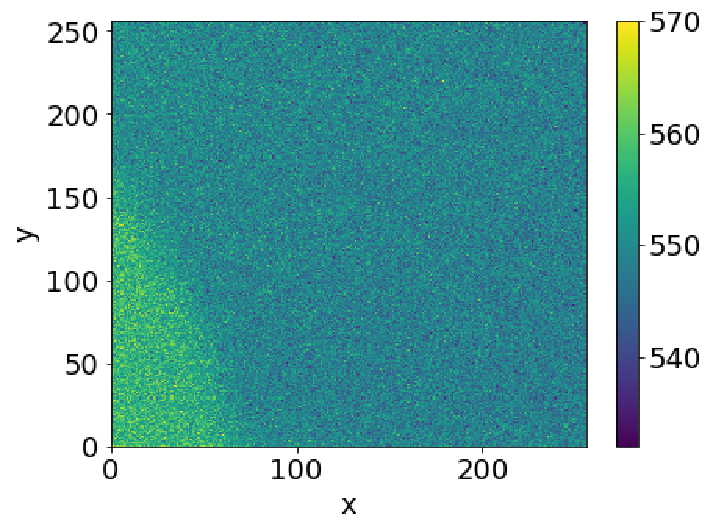
\includegraphics[scale=0.6]{figure/meikou_before.pdf}}
    \sidesubfloat[]{
        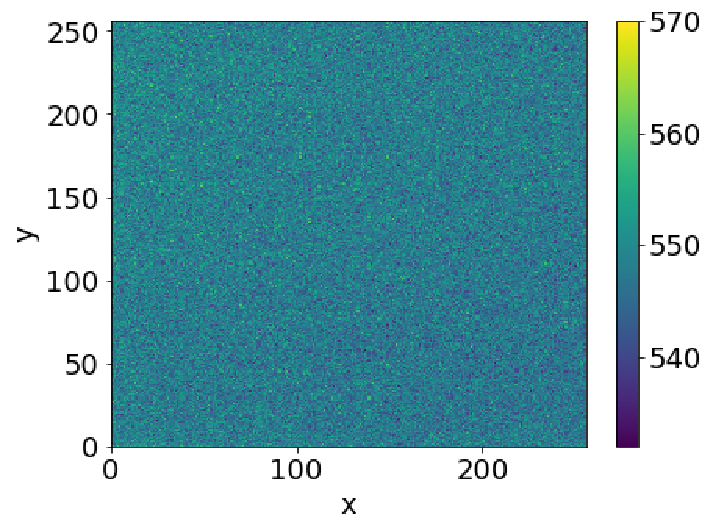
\includegraphics[scale=0.6]{figure/meikou_after.pdf}}
    \caption{遮光板を取り付け前後での迷光の様子.露光時間を1秒,x軸方向,y軸方向ともにビニングサイズを4で撮影した.
    (a)分光器内に遮光壁を取り付ける前に撮影したCCDカメラ受光部の光の強度分布,
    (b)分光器内に遮光壁を取り付けた後に撮影したCCDカメラ受光部の光の強度分布}
    \label{fig:meikou}
\end{figure}



\section{波長校正}
\label{sec:wavelength_calibration}
% 回折格子に入射された光は各波長ごとにx軸方向に分離され,CCDカメラに結像される.
% この際,得られたスペクトルに対応する光の波長は直接求めることはできず,そのスペクトルが得られる回折格子パルスしか分からない.
各スペクトルの波長を求めるためには回折格子パルスと波長の対応関係を求める必要がある.
He原子放電管を用いて$\pm{1}$次光及び0次光の各発光線がCCDカメラの中心部に結像されるような回折格子パルスを記録した.
これを既知のHe原子の各発光線の波長に対してプロットした(図\ \ref{fig:lambda-grating_fitting}).
\begin{figure}[htbp]
    \centering
    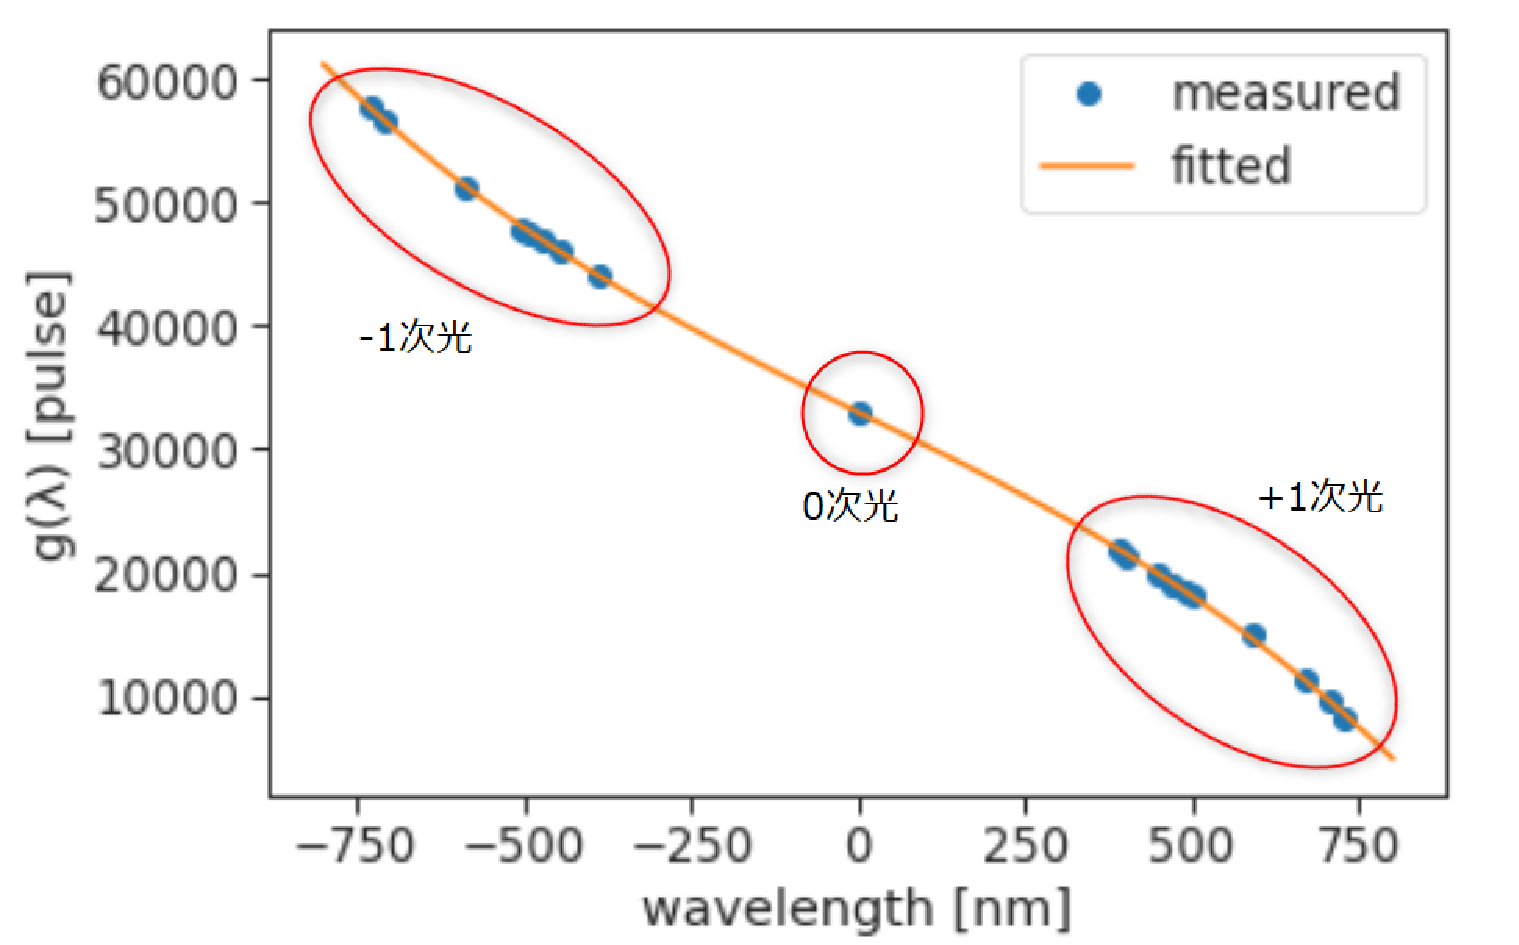
\includegraphics[scale=0.5]{figure/lambda-grating_fitting.pdf}
     \caption{波長と回折格子パルスの対応図.\\
     }
     \label{fig:lambda-grating_fitting}
\end{figure}
今回,グラフを作るために形式的に-1次光で計測したときの波長の値に-1を掛けて表示している.
波長$\lambda$のスペクトルが観測できる回折格子パルスの値$g(\lambda)$を$\lambda$の三次関数
\begin{equation}
     g(\lambda) = a\lambda^3+b\lambda^2+c\lambda+d
\end{equation}
でフィッテイングし,回折格子パルスと波長の対応関係を得た.




\section{色収差補正}
\label{sec:chromatic_aberration_correction}
% レンズを構成物質であるガラスの屈折率は波長によって異なる.
% そのため,レンズの焦点距離は波長によって変化してしまう.
% これを色収差と言い,レンズを使って光を集光させる場合,色収差を補正する必要がある.
単レンズと比べると小さいもののアクロマティックレンズにも色収差は存在する.
そのため,観測したい波長に応じてレンズの位置を調節する必要がある.
波長校正と同じく光源にHe原子放電管を用いて各発光線において図\ \ref{fig:HeNe_focus_example}(a)のような図を作成し,その発光線の波長とそれぞれで一番焦点が合っているフォーカスパルスの値を記録した.
観測波長の関数としてのフォーカスパルス$f(\lambda)$を$\pm{1}$次光それぞれにおいて
\begin{equation}
     f(\lambda) = a+b\lambda^2+c\frac{\lambda^2}{(\lambda^2-d)}
\end{equation}
でフィッテイングした.
図\ \ref{fig:lambda-focus_fitting}(a)(b)に$\pm{1}$次光における波長とフォーカスパルスの対応図を示す.
% これによって,波長とフォーカスパルスの対応関係が得られた.
\floatsetup[figure]{style=plain,subcapbesideposition=top}
\begin{figure}
    \sidesubfloat[]{
        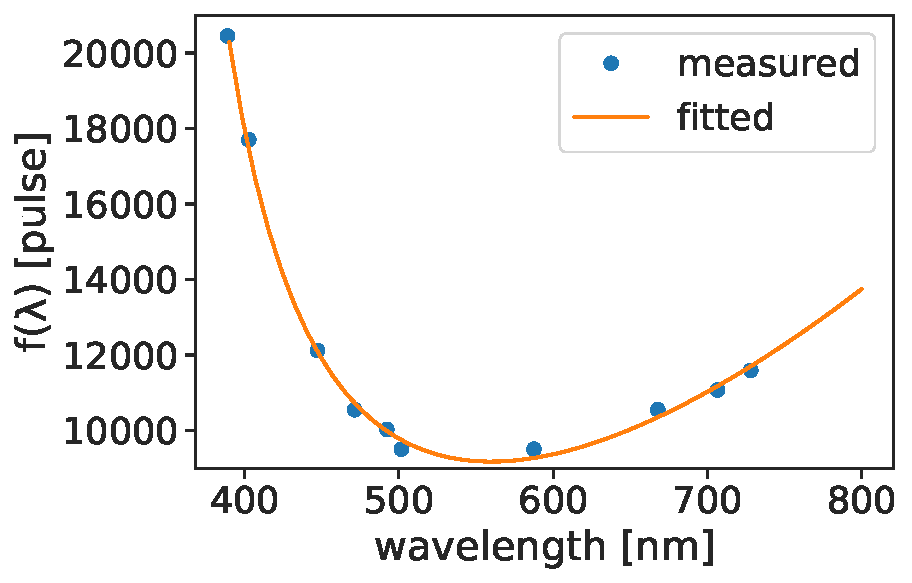
\includegraphics[scale=0.5]{figure/lambda-focus_fitting_1st.pdf}}
    \sidesubfloat[]{
        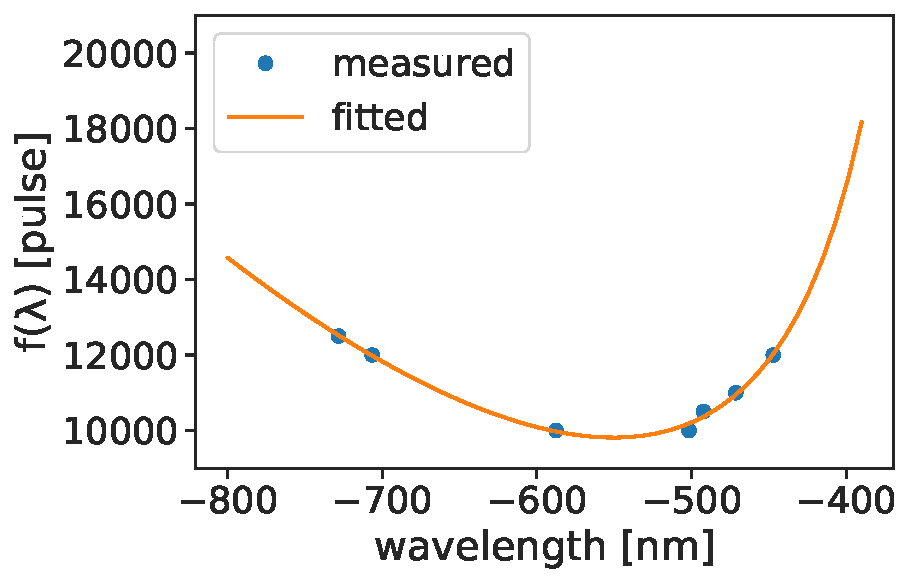
\includegraphics[scale=0.5]{figure/lambda-focus_fitting_-1st.pdf}}
    \caption{波長とフォーカスパルスの対応図\\
    (a)1次光における対応図,
    (b)-1次光における対応図}
    \label{fig:lambda-focus_fitting}
\end{figure}
% また,本実験で使用したアクロマティックレンズ(Edmund Optics TS 大口径アクロマティックレンズ 102 × 1525 枠付き)の色収差は性能データよりFig.\ \ref{fig:focal_shift_lense}のようになっている.
% \begin{figure}[htbp]
    % \centering
    % 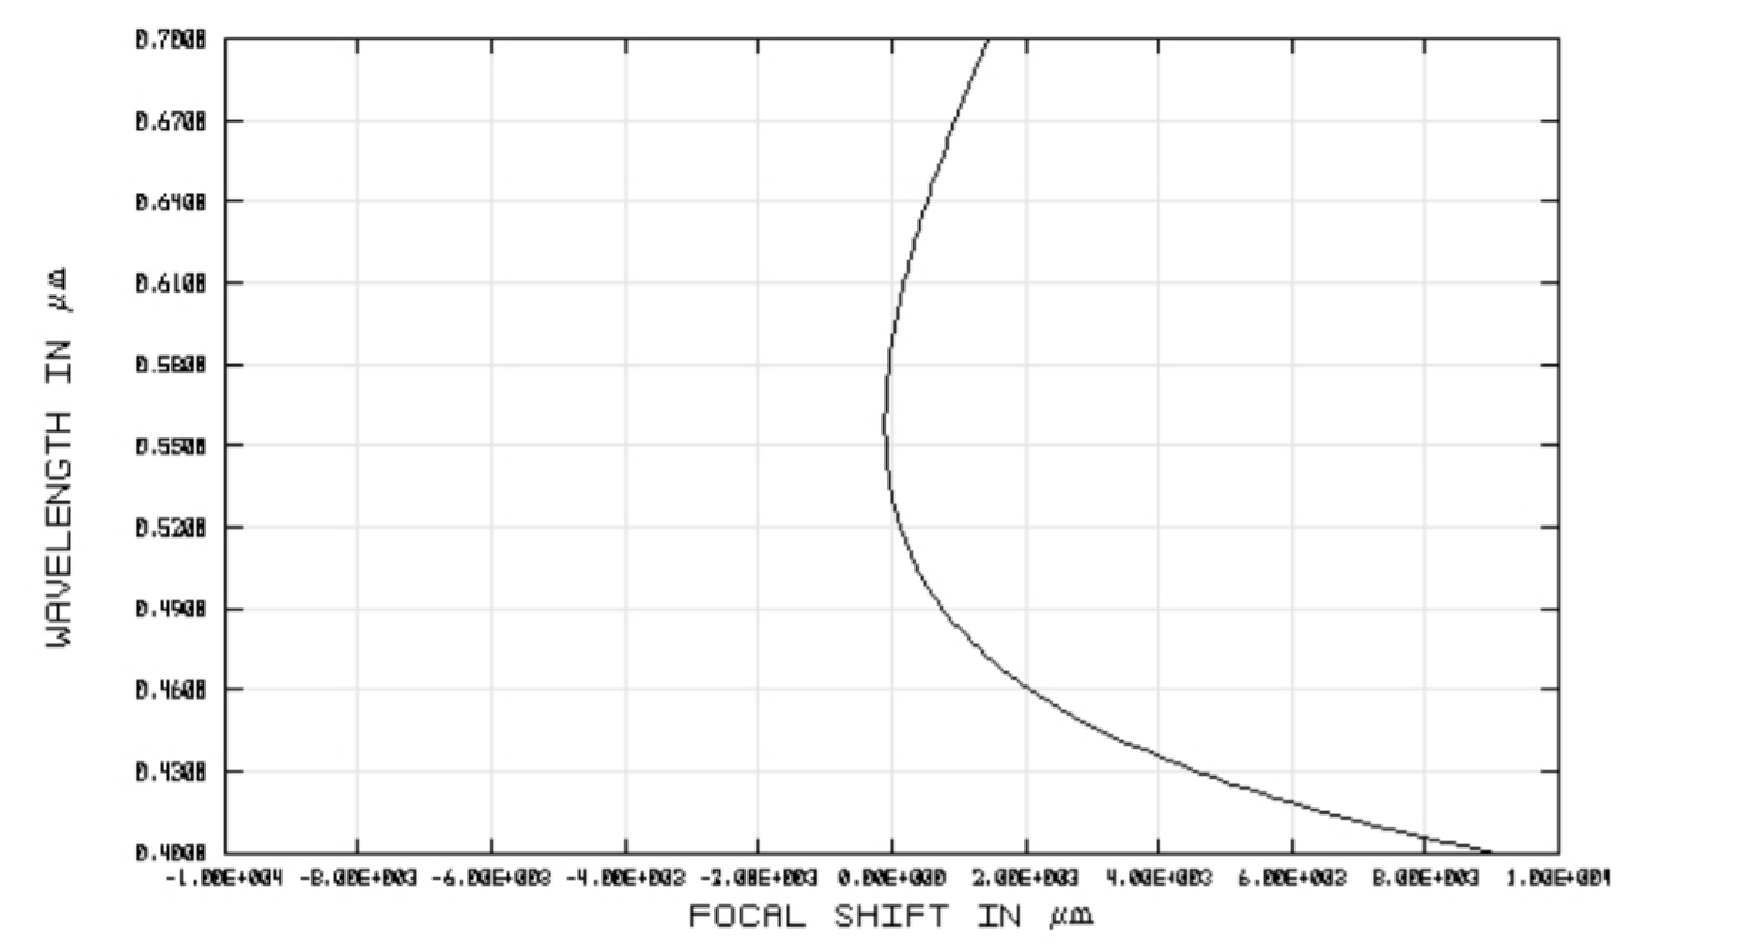
\includegraphics[scale=0.5]{figure/focal_shift_lense.pdf}
    % \caption{使用レンズの波長ごとの焦点シフト}
    % \label{fig:focal_shift_lense}
% \end{figure}
% Fig.\ \ref{fig:lambda-focus_fitting}ではレンズの設計通りの波長と焦点距離の関係を求めることができていると分かる.

前セクションの波長校正と合わせて,波長,回折格子パルス,フォーカスパルスの対応関係を得た.
これによって,欲しい波長範囲を指定することで回折格子パルス,フォーカスパルスが決定し制御できるようになった.
実際の実験ではPythonスクリプトによって自動回転ステージ,一軸自動ステージ及びCCDカメラの制御を行っている.
% ()に自動回転ステージ,一軸自動ステージの制御を行っているスクリプトの一例を示す.